\documentclass[]{article}
\usepackage{lmodern}
\usepackage{amssymb,amsmath}
\usepackage{ifxetex,ifluatex}
\usepackage{fixltx2e} % provides \textsubscript
\ifnum 0\ifxetex 1\fi\ifluatex 1\fi=0 % if pdftex
  \usepackage[T1]{fontenc}
  \usepackage[utf8]{inputenc}
\else % if luatex or xelatex
  \ifxetex
    \usepackage{mathspec}
  \else
    \usepackage{fontspec}
  \fi
  \defaultfontfeatures{Ligatures=TeX,Scale=MatchLowercase}
\fi
% use upquote if available, for straight quotes in verbatim environments
\IfFileExists{upquote.sty}{\usepackage{upquote}}{}
% use microtype if available
\IfFileExists{microtype.sty}{%
\usepackage{microtype}
\UseMicrotypeSet[protrusion]{basicmath} % disable protrusion for tt fonts
}{}
\usepackage[margin=1in]{geometry}
\usepackage{hyperref}
\hypersetup{unicode=true,
            pdftitle={lab1block2},
            pdfauthor={Prudhvi Peddmallu},
            pdfborder={0 0 0},
            breaklinks=true}
\urlstyle{same}  % don't use monospace font for urls
\usepackage{color}
\usepackage{fancyvrb}
\newcommand{\VerbBar}{|}
\newcommand{\VERB}{\Verb[commandchars=\\\{\}]}
\DefineVerbatimEnvironment{Highlighting}{Verbatim}{commandchars=\\\{\}}
% Add ',fontsize=\small' for more characters per line
\usepackage{framed}
\definecolor{shadecolor}{RGB}{248,248,248}
\newenvironment{Shaded}{\begin{snugshade}}{\end{snugshade}}
\newcommand{\KeywordTok}[1]{\textcolor[rgb]{0.13,0.29,0.53}{\textbf{#1}}}
\newcommand{\DataTypeTok}[1]{\textcolor[rgb]{0.13,0.29,0.53}{#1}}
\newcommand{\DecValTok}[1]{\textcolor[rgb]{0.00,0.00,0.81}{#1}}
\newcommand{\BaseNTok}[1]{\textcolor[rgb]{0.00,0.00,0.81}{#1}}
\newcommand{\FloatTok}[1]{\textcolor[rgb]{0.00,0.00,0.81}{#1}}
\newcommand{\ConstantTok}[1]{\textcolor[rgb]{0.00,0.00,0.00}{#1}}
\newcommand{\CharTok}[1]{\textcolor[rgb]{0.31,0.60,0.02}{#1}}
\newcommand{\SpecialCharTok}[1]{\textcolor[rgb]{0.00,0.00,0.00}{#1}}
\newcommand{\StringTok}[1]{\textcolor[rgb]{0.31,0.60,0.02}{#1}}
\newcommand{\VerbatimStringTok}[1]{\textcolor[rgb]{0.31,0.60,0.02}{#1}}
\newcommand{\SpecialStringTok}[1]{\textcolor[rgb]{0.31,0.60,0.02}{#1}}
\newcommand{\ImportTok}[1]{#1}
\newcommand{\CommentTok}[1]{\textcolor[rgb]{0.56,0.35,0.01}{\textit{#1}}}
\newcommand{\DocumentationTok}[1]{\textcolor[rgb]{0.56,0.35,0.01}{\textbf{\textit{#1}}}}
\newcommand{\AnnotationTok}[1]{\textcolor[rgb]{0.56,0.35,0.01}{\textbf{\textit{#1}}}}
\newcommand{\CommentVarTok}[1]{\textcolor[rgb]{0.56,0.35,0.01}{\textbf{\textit{#1}}}}
\newcommand{\OtherTok}[1]{\textcolor[rgb]{0.56,0.35,0.01}{#1}}
\newcommand{\FunctionTok}[1]{\textcolor[rgb]{0.00,0.00,0.00}{#1}}
\newcommand{\VariableTok}[1]{\textcolor[rgb]{0.00,0.00,0.00}{#1}}
\newcommand{\ControlFlowTok}[1]{\textcolor[rgb]{0.13,0.29,0.53}{\textbf{#1}}}
\newcommand{\OperatorTok}[1]{\textcolor[rgb]{0.81,0.36,0.00}{\textbf{#1}}}
\newcommand{\BuiltInTok}[1]{#1}
\newcommand{\ExtensionTok}[1]{#1}
\newcommand{\PreprocessorTok}[1]{\textcolor[rgb]{0.56,0.35,0.01}{\textit{#1}}}
\newcommand{\AttributeTok}[1]{\textcolor[rgb]{0.77,0.63,0.00}{#1}}
\newcommand{\RegionMarkerTok}[1]{#1}
\newcommand{\InformationTok}[1]{\textcolor[rgb]{0.56,0.35,0.01}{\textbf{\textit{#1}}}}
\newcommand{\WarningTok}[1]{\textcolor[rgb]{0.56,0.35,0.01}{\textbf{\textit{#1}}}}
\newcommand{\AlertTok}[1]{\textcolor[rgb]{0.94,0.16,0.16}{#1}}
\newcommand{\ErrorTok}[1]{\textcolor[rgb]{0.64,0.00,0.00}{\textbf{#1}}}
\newcommand{\NormalTok}[1]{#1}
\usepackage{graphicx,grffile}
\makeatletter
\def\maxwidth{\ifdim\Gin@nat@width>\linewidth\linewidth\else\Gin@nat@width\fi}
\def\maxheight{\ifdim\Gin@nat@height>\textheight\textheight\else\Gin@nat@height\fi}
\makeatother
% Scale images if necessary, so that they will not overflow the page
% margins by default, and it is still possible to overwrite the defaults
% using explicit options in \includegraphics[width, height, ...]{}
\setkeys{Gin}{width=\maxwidth,height=\maxheight,keepaspectratio}
\IfFileExists{parskip.sty}{%
\usepackage{parskip}
}{% else
\setlength{\parindent}{0pt}
\setlength{\parskip}{6pt plus 2pt minus 1pt}
}
\setlength{\emergencystretch}{3em}  % prevent overfull lines
\providecommand{\tightlist}{%
  \setlength{\itemsep}{0pt}\setlength{\parskip}{0pt}}
\setcounter{secnumdepth}{0}
% Redefines (sub)paragraphs to behave more like sections
\ifx\paragraph\undefined\else
\let\oldparagraph\paragraph
\renewcommand{\paragraph}[1]{\oldparagraph{#1}\mbox{}}
\fi
\ifx\subparagraph\undefined\else
\let\oldsubparagraph\subparagraph
\renewcommand{\subparagraph}[1]{\oldsubparagraph{#1}\mbox{}}
\fi

%%% Use protect on footnotes to avoid problems with footnotes in titles
\let\rmarkdownfootnote\footnote%
\def\footnote{\protect\rmarkdownfootnote}

%%% Change title format to be more compact
\usepackage{titling}

% Create subtitle command for use in maketitle
\newcommand{\subtitle}[1]{
  \posttitle{
    \begin{center}\large#1\end{center}
    }
}

\setlength{\droptitle}{-2em}

  \title{lab1block2}
    \pretitle{\vspace{\droptitle}\centering\huge}
  \posttitle{\par}
    \author{Prudhvi Peddmallu}
    \preauthor{\centering\large\emph}
  \postauthor{\par}
      \predate{\centering\large\emph}
  \postdate{\par}
    \date{23 April 2019}


\begin{document}
\maketitle

\section{1. ENSEMBLE METHODS}\label{ensemble-methods}

The file spambase.csv contains information about the frequency of
various words, characters, etc. for a total of 4601 e-mails.
Furthermore, these e-mails have been classified as spams (spam = 1) or
regular e-mails (spam = 0). You can find more information about these
data at. Your task is to evaluate the performance of Adaboost
classification trees and random forests on the spam data. Specifically,
provide a plot showing the error rates when the number of trees
considered are 10; 20; : : : ; 100. To estimate the error rates, use 2/3
of the data for training and 1/3 as hold-out test data.

To learn Adaboost classification trees, use the function blackboost() of
the R package mboost. Specify the loss function corresponding to
Adaboost with the parameter family. To learn random forests, use the
function randomForest of the R package randomForest. To load the data,
you may want to use the following code: sp \textless{}-
read.csv2(``spambase.csv'') sp\(Spam <- as.factor(sp\)Spam)

\subsection{Adaboost classification trees \&
randomForest.}\label{adaboost-classification-trees-randomforest.}

\begin{Shaded}
\begin{Highlighting}[]
\KeywordTok{library}\NormalTok{(mboost)}
\end{Highlighting}
\end{Shaded}

\begin{verbatim}
## Loading required package: parallel
\end{verbatim}

\begin{verbatim}
## Loading required package: stabs
\end{verbatim}

\begin{verbatim}
## This is mboost 2.9-1. See 'package?mboost' and 'news(package  = "mboost")'
## for a complete list of changes.
\end{verbatim}

\begin{Shaded}
\begin{Highlighting}[]
\KeywordTok{library}\NormalTok{(randomForest)}
\end{Highlighting}
\end{Shaded}

\begin{verbatim}
## randomForest 4.6-14
\end{verbatim}

\begin{verbatim}
## Type rfNews() to see new features/changes/bug fixes.
\end{verbatim}

\begin{Shaded}
\begin{Highlighting}[]
\KeywordTok{library}\NormalTok{(ggplot2)}
\end{Highlighting}
\end{Shaded}

\begin{verbatim}
## 
## Attaching package: 'ggplot2'
\end{verbatim}

\begin{verbatim}
## The following object is masked from 'package:randomForest':
## 
##     margin
\end{verbatim}

\begin{verbatim}
## The following object is masked from 'package:mboost':
## 
##     %+%
\end{verbatim}

\begin{Shaded}
\begin{Highlighting}[]
\NormalTok{sp <-}\StringTok{ }\KeywordTok{read.csv2}\NormalTok{(}\StringTok{"spambase.csv"}\NormalTok{)}
\NormalTok{sp}\OperatorTok{$}\NormalTok{Spam <-}\StringTok{ }\KeywordTok{as.factor}\NormalTok{(sp}\OperatorTok{$}\NormalTok{Spam)}
\NormalTok{n=}\KeywordTok{dim}\NormalTok{(sp)[}\DecValTok{1}\NormalTok{]}
\KeywordTok{set.seed}\NormalTok{(}\DecValTok{12345}\NormalTok{)}
\NormalTok{id=}\KeywordTok{sample}\NormalTok{(}\DecValTok{1}\OperatorTok{:}\NormalTok{n, }\KeywordTok{floor}\NormalTok{(n}\OperatorTok{*}\FloatTok{0.7}\NormalTok{))}
\NormalTok{sp_train=sp[id,]}
\NormalTok{sp_test=sp[}\OperatorTok{-}\NormalTok{id,]}
\NormalTok{n_trees <-}\StringTok{ }\KeywordTok{seq}\NormalTok{(}\DecValTok{10}\NormalTok{, }\DecValTok{100}\NormalTok{, }\DataTypeTok{by =} \DecValTok{10}\NormalTok{)}
\end{Highlighting}
\end{Shaded}

\begin{Shaded}
\begin{Highlighting}[]
\NormalTok{residualerror_ab <-}\StringTok{ }\KeywordTok{sapply}\NormalTok{(n_trees, }\ControlFlowTok{function}\NormalTok{(x)\{}
\NormalTok{model =}\StringTok{ }\KeywordTok{blackboost}\NormalTok{(Spam}\OperatorTok{~}\NormalTok{., sp_train,}
\DataTypeTok{family =} \KeywordTok{AdaExp}\NormalTok{(),}\DataTypeTok{control =} \KeywordTok{boost_control}\NormalTok{(}\DataTypeTok{mstop =}\NormalTok{ x))}
\NormalTok{yhat <-}\StringTok{ }\KeywordTok{predict}\NormalTok{(model, sp_test, }\DataTypeTok{type =} \StringTok{"class"}\NormalTok{)}
\NormalTok{c_matrix <-}\StringTok{ }\KeywordTok{table}\NormalTok{(yhat,sp_test}\OperatorTok{$}\NormalTok{Spam)}
\DecValTok{1}\OperatorTok{-}\NormalTok{(}\KeywordTok{sum}\NormalTok{(}\KeywordTok{diag}\NormalTok{(c_matrix))}\OperatorTok{/}\KeywordTok{sum}\NormalTok{(c_matrix))}
\NormalTok{\})}
\NormalTok{ab_errors <-}\StringTok{ }\KeywordTok{data.frame}\NormalTok{(}\StringTok{"ntrees"}\NormalTok{ =}\StringTok{ }\NormalTok{n_trees, }\StringTok{"error"}\NormalTok{ =}\StringTok{ }\NormalTok{residualerror_ab)}
\KeywordTok{ggplot}\NormalTok{(}\DataTypeTok{data =}\NormalTok{ ab_errors, }\KeywordTok{aes}\NormalTok{(}\DataTypeTok{x =}\NormalTok{ n_trees, }\DataTypeTok{y =}\NormalTok{ error))}\OperatorTok{+}\KeywordTok{geom_point}\NormalTok{()}\OperatorTok{+}\KeywordTok{geom_line}\NormalTok{() }\OperatorTok{+}
\KeywordTok{xlab}\NormalTok{(}\StringTok{"Number of Trees"}\NormalTok{) }\OperatorTok{+}\StringTok{ }\KeywordTok{ylab}\NormalTok{(}\StringTok{"Error"}\NormalTok{) }\OperatorTok{+}\StringTok{ }\KeywordTok{ggtitle}\NormalTok{(}\StringTok{"Number of Trees vs Error"}\NormalTok{)}
\end{Highlighting}
\end{Shaded}

\includegraphics{lab1block2_files/figure-latex/unnamed-chunk-2-1.pdf}

\begin{Shaded}
\begin{Highlighting}[]
\NormalTok{residualerror_rf <-}\StringTok{ }\KeywordTok{sapply}\NormalTok{(n_trees, }\ControlFlowTok{function}\NormalTok{(x)\{}
\NormalTok{model <-}\StringTok{ }\KeywordTok{randomForest}\NormalTok{(Spam}\OperatorTok{~}\NormalTok{., sp_train, }\DataTypeTok{importance=}\OtherTok{TRUE}\NormalTok{,}
\DataTypeTok{proximity=}\OtherTok{TRUE}\NormalTok{,}\DataTypeTok{ntree =}\NormalTok{ x)}
\NormalTok{yhat <-}\StringTok{ }\KeywordTok{predict}\NormalTok{(model, sp_test, }\DataTypeTok{type =} \StringTok{"class"}\NormalTok{)}
\NormalTok{c_matrix <-}\StringTok{ }\KeywordTok{table}\NormalTok{(yhat,sp_test}\OperatorTok{$}\NormalTok{Spam)}
\DecValTok{1}\OperatorTok{-}\NormalTok{(}\KeywordTok{sum}\NormalTok{(}\KeywordTok{diag}\NormalTok{(c_matrix))}\OperatorTok{/}\KeywordTok{sum}\NormalTok{(c_matrix))}
\NormalTok{\})}
\NormalTok{rf_errors <-}\StringTok{ }\KeywordTok{data.frame}\NormalTok{(}\StringTok{"ntrees"}\NormalTok{ =}\StringTok{ }\NormalTok{n_trees, }\StringTok{"error"}\NormalTok{ =}\StringTok{ }\NormalTok{residualerror_rf)}
\KeywordTok{ggplot}\NormalTok{(}\DataTypeTok{data =}\NormalTok{ rf_errors, }\KeywordTok{aes}\NormalTok{(}\DataTypeTok{x =}\NormalTok{ n_trees, }\DataTypeTok{y =}\NormalTok{ error))}\OperatorTok{+}\KeywordTok{geom_point}\NormalTok{()}\OperatorTok{+}\KeywordTok{geom_line}\NormalTok{() }\OperatorTok{+}
\KeywordTok{xlab}\NormalTok{(}\StringTok{"Number of Trees"}\NormalTok{) }\OperatorTok{+}\StringTok{ }\KeywordTok{ylab}\NormalTok{(}\StringTok{"Error"}\NormalTok{) }\OperatorTok{+}\StringTok{ }\KeywordTok{ggtitle}\NormalTok{(}\StringTok{"Number of Trees vs Error"}\NormalTok{)}
\end{Highlighting}
\end{Shaded}

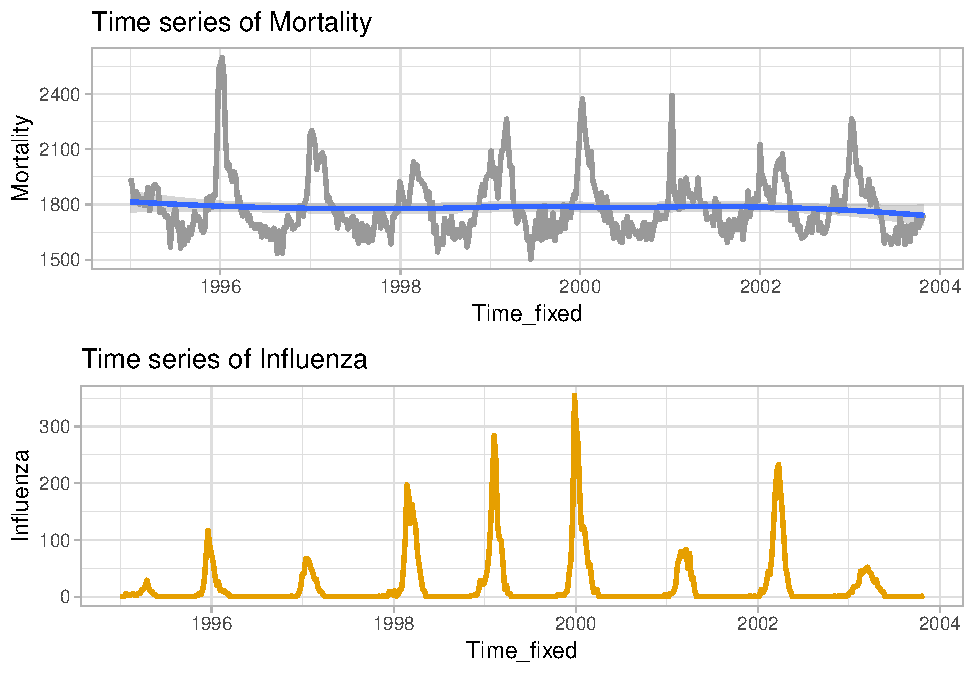
\includegraphics{lab1block2_files/figure-latex/unnamed-chunk-3-1.pdf}

\subsubsection{2-method}\label{method}

\subsection{Ada boost classification}\label{ada-boost-classification}

\begin{Shaded}
\begin{Highlighting}[]
\CommentTok{#libraries}
\KeywordTok{library}\NormalTok{(mboost)}
\end{Highlighting}
\end{Shaded}

\begin{Shaded}
\begin{Highlighting}[]
\CommentTok{# #Divideing the data into train(2/3=70%) and test(1/3=30%)}
\CommentTok{# n=dim(spambase)[1]}
\CommentTok{# set.seed(12345)}
\CommentTok{# id=sample(1:n, floor(n*0.7))}
\CommentTok{# train=spambase[id,]}
\CommentTok{# test=spambase[-id,]}
\end{Highlighting}
\end{Shaded}

\begin{Shaded}
\begin{Highlighting}[]
\CommentTok{# #Ada boost classification }
\CommentTok{# #loop for sequence to get order 10, 20, 30...100}
\CommentTok{# storeing<- c()}
\CommentTok{# sequences <- c()}
\CommentTok{# count<-0}
\CommentTok{#   for(i in seq(from=10, to=100 ,by =10))}
\CommentTok{#   \{ }
\CommentTok{#      sequences<-c(i,sequences)}
\CommentTok{# #fitting the model adaboost}
\CommentTok{# spambase_EM_fit <- blackboost(Spam~., data = train, family = AdaExp(),control = boost_control(mstop =i))}
\CommentTok{# #prediction we are giving type = class because the adaboost gives the tree contain the classes}
\CommentTok{# predectionEM_train <- predict(spambase_EM_fit,newdata=train,type='class')}
\CommentTok{# #confusion matrix}
\CommentTok{# confusionmatrix_trainEM = table(train$Spam,predectionEM_train)}
\CommentTok{# # misclassification errors according to i(10,20,30...)}
\CommentTok{# diagonal_trainEM<-diag(confusionmatrix_trainEM)}
\CommentTok{# summ_trainEM<-sum(confusionmatrix_trainEM)}
\CommentTok{# misclassificationrate_trainEM<-1-(sum(diagonal_trainEM)/sum(summ_trainEM))}
\CommentTok{# storeing<-c(misclassificationrate_trainEM,storeing)}
\CommentTok{# }
\CommentTok{# \}}
\CommentTok{# #plot the misclassification vs i}
\CommentTok{# \{plot(x=sequences,y=storeing,}
\CommentTok{# xlab="sequence models",}
\CommentTok{# ylab="misclassification errors"}
\CommentTok{# )}
\CommentTok{# lines(sequences,storeing,col="blue")\}}
\CommentTok{# ```}
\CommentTok{# ```\{r message=FALSE, warning=FALSE, paged.print=FALSE\}}
\CommentTok{# library(randomForest)}
\end{Highlighting}
\end{Shaded}

\begin{Shaded}
\begin{Highlighting}[]
\CommentTok{# #Divideing the data into train(2/3=70%) and test(1/3=30%)}
\CommentTok{# n=dim(spambase)[1]}
\CommentTok{# set.seed(12345)}
\CommentTok{# id=sample(1:n, floor(n*0.7))}
\CommentTok{# train_RF=spambase[id,]}
\CommentTok{# test_RF=spambase[-id,]}
\end{Highlighting}
\end{Shaded}

\subsection{Random forest}\label{random-forest}

\begin{Shaded}
\begin{Highlighting}[]
\CommentTok{# #Random forest}
\CommentTok{# storeing_RF<-c()}
\CommentTok{# sequences_RF<-c()}
\CommentTok{# count<-0}
\CommentTok{# for(i in seq(from=10,to=100,by=10))\{}
\CommentTok{#  sequences_RF<-c(i,sequences_RF)}
\CommentTok{# #fitting the model adaboost}
\CommentTok{# spambase_RF_fit <- randomForest(Spam~., data = train_RF,control = boost_control(mstop =i))}
\CommentTok{# #prediction we are giving type = class because the adaboost gives the tree contain the classes}
\CommentTok{# predectionRF_train <- predict(spambase_RF_fit,newdata=train_RF,type='class')}
\CommentTok{# #confusion matrix}
\CommentTok{# confusionmatrix_trainRF = table(train_RF$Spam,predectionRF_train)}
\CommentTok{# # misclassification errors according to i(10,20,30...)}
\CommentTok{# diagonal_trainRF<-diag(confusionmatrix_trainRF)}
\CommentTok{# summ_trainRF<-sum(confusionmatrix_trainRF)}
\CommentTok{# misclassificationrate_trainRF<-1-(sum(diagonal_trainRF)/sum(summ_trainRF))}
\CommentTok{# storeing_RF<-c(misclassificationrate_trainRF,storeing_RF)}
\CommentTok{# \}}
\CommentTok{# #plot the misclassification vs i}
\CommentTok{# \{plot(x=sequences_RF,y=storeing_RF,}
\CommentTok{# xlab="sequence models-RF",}
\CommentTok{# ylab="misclassification errors"}
\CommentTok{# )}
\CommentTok{# lines(sequences_RF,storeing_RF,col="purple")  \}}
\end{Highlighting}
\end{Shaded}

\subsection{2-method-Adaboost classification trees \&
randomForest.}\label{method-adaboost-classification-trees-randomforest.}

Loading Input files

\begin{Shaded}
\begin{Highlighting}[]
\CommentTok{# spam_data <- read.csv(file = "spambase.data", header = FALSE)}
\CommentTok{# colnames(spam_data)[58] <- "Spam"}
\CommentTok{# spam_data$Spam <- factor(spam_data$Spam, levels = c(0,1), labels = c("0", "1"))}
\end{Highlighting}
\end{Shaded}

Splitting into Train and Test with 66\% and 33\% ratio.

\begin{Shaded}
\begin{Highlighting}[]
\CommentTok{# set.seed(12345)}
\CommentTok{# n =  NROW(spam_data)}
\CommentTok{# id = sample(1:n, floor(n*(2/3)))}
\CommentTok{# train = spam_data[id,]}
\CommentTok{# test = spam_data[-id,]}
\end{Highlighting}
\end{Shaded}

Trainning the Model

\subsubsection{Adaboost with varying
depth}\label{adaboost-with-varying-depth}

\begin{Shaded}
\begin{Highlighting}[]
\CommentTok{# final_result <- NULL}
\CommentTok{# for(i in seq(from = 10, to = 100, by = 10))\{}
\CommentTok{# ada_model <- mboost::blackboost(Spam~., }
\CommentTok{#                                  data = train, }
\CommentTok{#                                  family = AdaExp(), }
\CommentTok{#                                control=boost_control(mstop=i))}
\CommentTok{# forest_model <- randomForest(Spam~., data = train, ntree = i)}
\CommentTok{# prediction_function <- function(model, data)\{}
\CommentTok{#   predicted <- predict(model, newdata = data, type = c("class"))}
\CommentTok{#   predict_correct <- ifelse(data$Spam == predicted, 1, 0) }
\CommentTok{#   score <- sum(predict_correct)/NROW(data)}
\CommentTok{#   return(score)}
\CommentTok{# \}}
\CommentTok{# train_ada_model_predict <- predict(ada_model, newdata = train, type = c("class"))}
\CommentTok{# test_ada_model_predict <- predict(ada_model, newdata = test, type = c("class"))}
\CommentTok{# train_forest_model_predict <- predict(forest_model, newdata = train, type = c("class"))}
\CommentTok{# test_forest_model_predict <- predict(forest_model, newdata = test, type = c("class"))}
\CommentTok{# test_predict_correct <- ifelse(test$Spam == test_forest_model_predict, 1, 0) }
\CommentTok{# train_predict_correct <- ifelse(train$Spam == train_forest_model_predict, 1, 0) }
\CommentTok{# train_ada_score <-  prediction_function(ada_model, train)}
\CommentTok{# test_ada_score <-  prediction_function(ada_model, test)}
\CommentTok{# train_forest_score <-  prediction_function(forest_model, train)}
\CommentTok{# test_forest_score <-  prediction_function(forest_model, test)}
\CommentTok{# iteration_result <- data.frame(number_of_trees = i, }
\CommentTok{#                                accuracy = c(train_ada_score, }
\CommentTok{#                                             test_ada_score, }
\CommentTok{#                                             train_forest_score, }
\CommentTok{#                                             test_forest_score), }
\CommentTok{#                                type  = c("train", "test", "train", "test"),}
\CommentTok{#                                model = c("ADA", "ADA",  "Forest", "Forest"))}
\CommentTok{# final_result <- rbind(iteration_result, final_result)}
\CommentTok{# \}}
\CommentTok{# final_result$error_rate_percentage <- 100*(1 - final_result$accuracy)}
\CommentTok{# ggplot(data = final_result, aes(x = number_of_trees, }
\CommentTok{#                                 y = error_rate_percentage, }
\CommentTok{#                                 group = type, color = type)) + }
\CommentTok{#   geom_point() + }
\CommentTok{#   geom_line() + }
\CommentTok{#   ggtitle("Error Rate vs. increase in trees") + facet_grid(rows = vars(model))}
\end{Highlighting}
\end{Shaded}

\section{2. MIXTURE MODELS-EM}\label{mixture-models-em}

Your task is to implement the EM algorithm for mixtures of multivariate
Benoulli distributions. Please use the template in the next page to
solve the assignment. Then, use your implementation to show what happens
when your mixture models has too few and too many components, i.e.~set K
= 2; 3; 4 and compare results. Please provide a short explanation as
well.

\paragraph{Given question code}\label{given-question-code}

\begin{Shaded}
\begin{Highlighting}[]
\CommentTok{# set.seed(1234567890)}
\CommentTok{# max_it <- 100 # max number of EM iterations}
\CommentTok{# min_change <- 0.1 # min change in log likelihood between two consecutive EM iterations}
\CommentTok{# N=1000 # number of training points}
\CommentTok{# D=10 # number of dimensions}
\CommentTok{# x <- matrix(nrow=N, ncol=D) # training data}
\CommentTok{# true_pi <- vector(length = 3) # true mixing coefficients}
\CommentTok{# true_mu <- matrix(nrow=3, ncol=D) # true conditional distributions}
\CommentTok{# true_pi=c(1/3, 1/3, 1/3)}
\CommentTok{# true_mu[1,]=c(0.5,0.6,0.4,0.7,0.3,0.8,0.2,0.9,0.1,1)}
\CommentTok{# true_mu[2,]=c(0.5,0.4,0.6,0.3,0.7,0.2,0.8,0.1,0.9,0)}
\CommentTok{# true_mu[3,]=c(0.5,0.5,0.5,0.5,0.5,0.5,0.5,0.5,0.5,0.5)}
\CommentTok{# plot(true_mu[1,], type="o", col="blue", ylim=c(0,1))}
\CommentTok{# points(true_mu[2,], type="o", col="red")}
\CommentTok{# points(true_mu[3,], type="o", col="green")}
\CommentTok{# # Producing the training data}
\CommentTok{# for(n in 1:N) \{}
\CommentTok{# k <- sample(1:3,1,prob=true_pi)}
\CommentTok{# for(d in 1:D) \{}
\CommentTok{# x[n,d] <- rbinom(1,1,true_mu[k,d])}
\CommentTok{# \}}
\CommentTok{# \}}
\CommentTok{# K=3 # number of guessed components}
\CommentTok{# z <- matrix(nrow=N, ncol=K) # fractional component assignments}
\CommentTok{# pi <- vector(length = K) # mixing coefficients}
\CommentTok{# mu <- matrix(nrow=K, ncol=D) # conditional distributions}
\CommentTok{# llik <- vector(length = max_it) # log likelihood of the EM iterations}
\CommentTok{# # Random initialization of the paramters}
\CommentTok{# pi <- runif(K,0.49,0.51)}
\CommentTok{# pi <- pi / sum(pi)}
\CommentTok{# for(k in 1:K) \{}
\CommentTok{# mu[k,] <- runif(D,0.49,0.51)}
\CommentTok{# \}}
\CommentTok{# pi}
\CommentTok{# mu}
\CommentTok{# for(it in 1:max_it) \{}
\CommentTok{# plot(mu[1,], type="o", col="blue", ylim=c(0,1))}
\CommentTok{# points(mu[2,], type="o", col="red")}
\CommentTok{# points(mu[3,], type="o", col="green")}
\CommentTok{# #points(mu[4,], type="o", col="yellow")}
\CommentTok{# Sys.sleep(0.5)}
\CommentTok{# # E-step: Computation of the fractional component assignments}
\CommentTok{# # Your code here}
\CommentTok{# #Log likelihood computation.}
\CommentTok{# # Your code here}
\CommentTok{# cat("iteration: ", it, "log likelihood: ", llik[it], "\textbackslash{}n")}
\CommentTok{# flush.console()}
\CommentTok{# # Stop if the lok likelihood has not changed significantly}
\CommentTok{# # Your code here}
\CommentTok{# #M-step: ML parameter estimation from the data and fractional component assignments}
\CommentTok{# # Your code here}
\CommentTok{# \}}
\CommentTok{# pi}
\CommentTok{# mu}
\CommentTok{# plot(llik[1:it], type="o")}
\end{Highlighting}
\end{Shaded}

\subsubsection{Code}\label{code}

To compare the results for K = 2,3,4, the em\_loop-function provides a
graphical analysis for every iteration. The function includes comments
which explain what I did at which step to create the EM algorithm. The
function will be finally run with K = 2,3,4.

\begin{Shaded}
\begin{Highlighting}[]
\CommentTok{# em_loop = function(K) \{}
\CommentTok{# # Initializing data}
\CommentTok{# set.seed(1234567890)}
\CommentTok{# max_it = 100 # max number of EM iterations}
\CommentTok{# min_change = 0.1 # min change in log likelihood between two consecutive EM iterations}
\CommentTok{# N = 1000 # number of training points}
\CommentTok{# D = 10 # number of dimensions}
\CommentTok{# x = matrix(nrow=N, ncol = D) # training data}
\CommentTok{# true_pi = vector(length = K) # true mixing coefficients}
\CommentTok{# true_mu = matrix(nrow = K, ncol = D) # true conditional distributions}
\CommentTok{# true_pi = c(rep(1/K, K))}
\CommentTok{# if (K == 2) \{}
\CommentTok{# true_mu[1,] = c(0.5,0.6,0.4,0.7,0.3,0.8,0.2,0.9,0.1,1)}
\CommentTok{# true_mu[2,] = c(0.5,0.4,0.6,0.3,0.7,0.2,0.8,0.1,0.9,0)}
\CommentTok{# plot(true_mu[1,], type = "o", xlab = "dimension", col = "blue",}
\CommentTok{# ylim = c(0,1), main = "True")}
\CommentTok{# points(true_mu[2,], type="o", xlab = "dimension", col = "red",}
\CommentTok{# main = "True")}
\CommentTok{# \} else if (K == 3) \{}
\CommentTok{# true_mu[1,] = c(0.5,0.6,0.4,0.7,0.3,0.8,0.2,0.9,0.1,1)}
\CommentTok{# true_mu[2,] = c(0.5,0.4,0.6,0.3,0.7,0.2,0.8,0.1,0.9,0)}
\CommentTok{# true_mu[3,] = c(0.5,0.5,0.5,0.5,0.5,0.5,0.5,0.5,0.5,0.5)}
\CommentTok{# plot(true_mu[1,], type = "o", xlab = "dimension", col = "blue", ylim=c(0,1),}
\CommentTok{# main = "True")}
\CommentTok{# points(true_mu[2,], type = "o", xlab = "dimension", col = "red",}
\CommentTok{# main = "True")}
\CommentTok{# points(true_mu[3,], type = "o", xlab = "dimension", col = "green",}
\CommentTok{# main = "True")}
\CommentTok{# \} else \{}
\CommentTok{# true_mu[1,] = c(0.5,0.6,0.4,0.7,0.3,0.8,0.2,0.9,0.1,1)}
\CommentTok{# true_mu[2,] = c(0.5,0.4,0.6,0.3,0.7,0.2,0.8,0.1,0.9,0)}
\CommentTok{# true_mu[3,] = c(0.5,0.5,0.5,0.5,0.5,0.5,0.5,0.5,0.5,0.5)}
\CommentTok{# true_mu[4,] = c(0.3,0.5,0.5,0.7,0.5,0.5,0.5,0.5,0.4,0.5)}
\CommentTok{# plot(true_mu[1,], type = "o", xlab = "dimension", col = "blue",}
\CommentTok{# ylim = c(0,1), main = "True")}
\CommentTok{# points(true_mu[2,], type = "o", xlab = "dimension", col = "red",}
\CommentTok{# main = "True")}
\CommentTok{# points(true_mu[3,], type = "o", xlab = "dimension", col = "green",}
\CommentTok{# main = "True")}
\CommentTok{# points(true_mu[4,], type = "o", xlab = "dimension", col = "yellow",}
\CommentTok{# main = "True")}
\CommentTok{# \}}
\CommentTok{# z = matrix(nrow = N, ncol = K) # fractional component assignments}
\CommentTok{# pi = vector(length = K) # mixing coefficients}
\CommentTok{# mu = matrix(nrow = K, ncol = D) # conditional distributions}
\CommentTok{# llik = vector(length = max_it) # log likelihood of the EM iterations}
\CommentTok{# # Producing the training data}
\CommentTok{# for(n in 1:N) \{}
\CommentTok{# k = sample(1:K, 1, prob=true_pi)}
\CommentTok{# for(d in 1:D) \{}
\CommentTok{# x[n,d] = rbinom(1, 1, true_mu[k,d])}
\CommentTok{# \}}
\CommentTok{# \}}
\CommentTok{# # Random initialization of the paramters}
\CommentTok{# pi = runif(K, 0.49, 0.51)}
\CommentTok{# pi = pi / sum(pi)}
\CommentTok{# for(k in 1:K) \{}
\CommentTok{# mu[k,] = runif(D, 0.49, 0.51)}
\CommentTok{# \}}
\CommentTok{# #EM algorithm}
\CommentTok{# for(it in 1:max_it) \{}
\CommentTok{# # Plotting mu}
\CommentTok{# # Defining plot title}
\CommentTok{# title = paste0("Iteration", it)}
\CommentTok{# if (K == 2) \{}
\CommentTok{# plot(mu[1,], type = "o", xlab = "dimension", col = "blue", ylim = c(0,1), main = title)}
\CommentTok{# points(mu[2,], type = "o", xlab = "dimension", col = "red", main = title)}
\CommentTok{# \} else if (K == 3) \{}
\CommentTok{# plot(mu[1,], type = "o", xlab = "dimension", col = "blue", ylim = c(0,1), main = title)}
\CommentTok{# points(mu[2,], type = "o", xlab = "dimension", col = "red", main = title)}
\CommentTok{# points(mu[3,], type = "o", xlab = "dimension", col = "green", main = title)}
\CommentTok{# \} else \{}
\CommentTok{# plot(mu[1,], type = "o", xlab = "dimension", col = "blue", ylim = c(0,1), main = title)}
\CommentTok{# points(mu[2,], type = "o", xlab = "dimension", col = "red", main = title)}
\CommentTok{# points(mu[3,], type = "o", xlab = "dimension", col = "green", main = title)}
\CommentTok{# points(mu[4,], type = "o", xlab = "dimension", col = "yellow", main = title)}
\CommentTok{# \}}
\CommentTok{# Sys.sleep(0.5)}
\CommentTok{# # E-step: Computation of the fractional component assignments}
\CommentTok{# for (n in 1:N) \{}
\CommentTok{# # Creating empty matrix (column 1:K = p_x_given_k; column K+1 = p(x|all k)}
\CommentTok{# p_x = matrix(data = c(rep(1,K), 0), nrow = 1, ncol = K+1)}
\CommentTok{# # Calculating p(x|k) and p(x|all k)}
\CommentTok{# for (k in 1:K) \{}
\CommentTok{# # Calculating p(x|k)}
\CommentTok{# for (d in 1:D) \{}
\CommentTok{# p_x[1,k] = p_x[1,k] * (mu[k,d]^x[n,d]) * (1-mu[k,d])^(1-x[n,d])}
\CommentTok{# \}}
\CommentTok{# p_x[1,k] = p_x[1,k] * pi[k] # weighting with pi[k]}
\CommentTok{# # Calculating p(x|all k) (denominator)}
\CommentTok{# p_x[1,K+1] = p_x[1,K+1] + p_x[1,k]}
\CommentTok{# \}}
\CommentTok{# # Calculating z for n and all k}
\CommentTok{# for (k in 1:K) \{}
\CommentTok{# z[n,k] = p_x[1,k] / p_x[1,K+1]}
\CommentTok{# \}}
\CommentTok{# \}}
\CommentTok{# # Log likelihood computation}
\CommentTok{# for (n in 1:N) \{}
\CommentTok{# for (k in 1:K) \{}
\CommentTok{# log_term = 0}
\CommentTok{# for (d in 1:D) \{}
\CommentTok{# log_term = log_term + x[n,d] * log(mu[k,d]) + (1-x[n,d]) * log(1-mu[k,d])}
\CommentTok{# \}}
\CommentTok{# llik[it] = llik[it] + z[n,k] * (log(pi[k]) + log_term)}
\CommentTok{# \}}
\CommentTok{# \}}
\CommentTok{# cat("iteration: ", it, "log likelihood: ", llik[it], "\textbackslash{}n")}
\CommentTok{# flush.console()}
\CommentTok{# # Stop if the log likelihood has not changed significantly}
\CommentTok{# if (it != 1) \{}
\CommentTok{# if (abs(llik[it] - llik[it-1]) < min_change) \{}
\CommentTok{# break}
\CommentTok{# \}}
\CommentTok{# \}}
\CommentTok{# # M-step: ML parameter estimation from the data and fractional component assignments}
\CommentTok{# # Updating pi}
\CommentTok{# for (k in 1:K) \{}
\CommentTok{# pi[k] = sum(z[,k])/N}
\CommentTok{# \}}
\CommentTok{# # Updating mu}
\CommentTok{# for (k in 1:K) \{}
\CommentTok{# mu[k,] = 0}
\CommentTok{# for (n in 1:N) \{}
\CommentTok{#   mu[k,] = mu[k,] + x[n,] * z[n,k]}
\CommentTok{# \}}
\CommentTok{# mu[k,] = mu[k,] / sum(z[,k])}
\CommentTok{# \}}
\CommentTok{# \}}
\CommentTok{# # Printing pi, mu and development of log likelihood at the end}
\CommentTok{# return(list(}
\CommentTok{# pi = pi,}
\CommentTok{# mu = mu,}
\CommentTok{# logLikelihoodDevelopment = plot(llik[1:it],}
\CommentTok{# type = "o",}
\CommentTok{# main = "Development of the log likelihood",}
\CommentTok{# xlab = "iteration",}
\CommentTok{# ylab = "log likelihood")}
\CommentTok{# ))}
\CommentTok{# \}}
\CommentTok{# ```}
\CommentTok{# }
\NormalTok{### K=2}
\CommentTok{# ```\{r, out.width='40%', fig.align = "center" \}}
\CommentTok{# em_loop(2)}
\end{Highlighting}
\end{Shaded}

\paragraph{K=3}\label{k3}

\begin{Shaded}
\begin{Highlighting}[]
\NormalTok{## K=3}
\CommentTok{#em_loop(3)}
\end{Highlighting}
\end{Shaded}

\paragraph{K=4}\label{k4}

\begin{Shaded}
\begin{Highlighting}[]
\CommentTok{#em_loop(4)}
\end{Highlighting}
\end{Shaded}

\paragraph{Analysis}\label{analysis}

Comparing the final plots for each of the cases, it becomes clear that
when the mixture model has more components (K = 4), the EM algorithm
does not perform as accurate as for fewer components (K = 2 or K = 3).
The segregation between each component gets diluted as the components
get higher.

\section{EM algo with matrix}\label{em-algo-with-matrix}

\begin{Shaded}
\begin{Highlighting}[]
\CommentTok{# em_mat <- function(k)\{}
\CommentTok{# set.seed(1234567890)}
\CommentTok{# # max number of EM iterations}
\CommentTok{# max_it <- 100}
\CommentTok{# # min change in log likelihood between two consecutive EM iterations}
\CommentTok{# min_change <- 0.1}
\CommentTok{# #------------- Producing Training data and Initialization ----------------#}
\CommentTok{# # number of training points}
\CommentTok{# N <- 1000}
\CommentTok{# # number of dimensions}
\CommentTok{# D <- 10}
\CommentTok{# # training data}
\CommentTok{# x <- matrix(nrow=N, ncol=D)}
\CommentTok{# # true mixing coefficients}
\CommentTok{# true_pi <- vector(length = k)}
\CommentTok{# true_pi <- rep(1/k, k)}
\CommentTok{# # true conditional distributions}
\CommentTok{# true_mu <- matrix(nrow = k, ncol = D)}
\CommentTok{# if(k == 2)\{}
\CommentTok{# plot(true_mu[1,], type="o", col="blue", ylim=c(0,1))}
\CommentTok{# points(true_mu[2,], type="o", col="red")}
\CommentTok{# true_mu[1,]=c(0.5,0.6,0.4,0.7,0.3,0.8,0.2,0.9,0.1,1)}
\CommentTok{# true_mu[2,]=c(0.5,0.4,0.6,0.3,0.7,0.2,0.8,0.1,0.9,0)}
\CommentTok{# \}else if(k == 3)\{}
\CommentTok{# plot(true_mu[1,], type="o", col="blue", ylim=c(0,1))}
\CommentTok{# points(true_mu[2,], type="o", col="red")}
\CommentTok{# points(true_mu[3,], type="o", col="green")}
\CommentTok{# true_mu[1,]=c(0.5,0.6,0.4,0.7,0.3,0.8,0.2,0.9,0.1,1)}
\CommentTok{# true_mu[2,]=c(0.5,0.4,0.6,0.3,0.7,0.2,0.8,0.1,0.9,0)}
\CommentTok{# true_mu[3,]=c(0.5,0.5,0.5,0.5,0.5,0.5,0.5,0.5,0.5,0.5)}
\CommentTok{# \}else \{}
\CommentTok{# plot(true_mu[1,], type="o", col="blue", ylim=c(0,1))}
\CommentTok{# points(true_mu[2,], type="o", col="red")}
\CommentTok{# points(true_mu[3,], type="o", col="green")}
\CommentTok{# points(true_mu[4,], type="o", col="yellow")}
\CommentTok{# true_mu[1,]=c(0.5,0.6,0.4,0.7,0.3,0.8,0.2,0.9,0.1,1)}
\CommentTok{# true_mu[2,]=c(0.5,0.4,0.6,0.3,0.7,0.2,0.8,0.1,0.9,0)}
\CommentTok{# true_mu[3,]=c(0.5,0.5,0.5,0.5,0.5,0.5,0.5,0.5,0.5,0.5)}
\CommentTok{# true_mu[4,]=c(0.3,0.5,0.5,0.7,0.5,0.5,0.5,0.5,0.4,0.5)\}}
\CommentTok{# # Producing the training data}
\CommentTok{# for(n in 1:N) \{}
\CommentTok{# l <- sample(1:k,1,prob=true_pi)}
\CommentTok{# for(d in 1:D) \{}
\CommentTok{# x[n,d] <- rbinom(1,1,true_mu[l,d])}
\CommentTok{# \}}
\CommentTok{# \}}
\CommentTok{# # fractional component assignments}
\CommentTok{# z <- matrix(nrow = N, ncol = k)}
\CommentTok{# # mixing coefficients}
\CommentTok{# pi <- vector(length = k)}
\CommentTok{# # conditional distributions}
\CommentTok{# mu <- matrix(nrow = k, ncol = D)}
\CommentTok{# # log likelihood of the EM iterations}
\CommentTok{# llik <- vector(length = max_it)}
\CommentTok{# # Random initialization of the paramters}
\CommentTok{# pi <- runif(k,0.49,0.51)}
\CommentTok{# pi <- pi / sum(pi)}
\CommentTok{# for(i in 1:k) \{}
\CommentTok{# mu[i,] <- runif(D,0.49,0.51)}
\CommentTok{# \}}
\CommentTok{# #----------------------- Iteration stage -----------------------#}
\CommentTok{# for(it in 1:max_it) \{}
\CommentTok{# if(k == 2)\{}
\CommentTok{# plot(mu[1,], type="o", col="blue", ylim=c(0,1))}
\CommentTok{# points(mu[2,], type="o", col="red")}
\CommentTok{# \}else if(k == 3)\{}
\CommentTok{# plot(mu[1,], type="o", col="blue", ylim=c(0,1))}
\CommentTok{# points(mu[2,], type="o", col="red")}
\CommentTok{# points(mu[3,], type="o", col="green")}
\CommentTok{# \}else\{}
\CommentTok{# plot(mu[1,], type="o", col="blue", ylim=c(0,1))}
\CommentTok{# points(mu[2,], type="o", col="red")}
\CommentTok{# points(mu[3,], type="o", col="green")}
\CommentTok{# points(mu[4,], type="o", col="yellow")\}}
\CommentTok{# Sys.sleep(0.5)}
\CommentTok{# # E-step: Computation of the fractional component assignments}
\CommentTok{# # Updating z matrix}
\CommentTok{# p_Xn_MUn <- exp(x %*% log(t(mu)) + (1 - x) %*% log(1 - t(mu)))}
\CommentTok{# numerator <- matrix(rep(pi,N), ncol = k, byrow = TRUE) * p_Xn_MUn}
\CommentTok{# denominator <- rowSums(numerator)}
\CommentTok{# Z_nk <- numerator/denominator}
\CommentTok{# # Updating pi}
\CommentTok{# pi <- colSums(Z_nk)/N}
\CommentTok{# # Updating mu}
\CommentTok{# mu <- (t(Z_nk) %*% x)/colSums(Z_nk)}
\CommentTok{# #Log likelihood computation.}
\CommentTok{# llik[it] <- sum(Z_nk * ((x %*% log(t(mu)) + (1 - x) %*% log(1 - t(mu))}
\CommentTok{# ) + matrix(rep(pi,N), ncol = k, byrow = TRUE)))}
\CommentTok{# cat("iteration: ", it, "log likelihood: ", llik[it], "\textbackslash{}n")}
\CommentTok{# flush.console()}
\CommentTok{# # Stop if the log likelihood has not changed significantly}
\CommentTok{# if(it >= 2)\{}
\CommentTok{# if((llik[it] - llik[it-1]) < min_change)\{break()\}}
\CommentTok{# \}}
\CommentTok{# #M-step: ML parameter estimation from the data and fractional component assignments}
\CommentTok{# # pi_ML}
\CommentTok{# pi_ML <- pi}
\CommentTok{# #mu_ML}
\CommentTok{# mu_ML <- mu}
\CommentTok{# \}}
\CommentTok{# #----------------------- output stage -----------------------#}
\CommentTok{# df <- data.frame(Iteration = 1:length(llik[which(llik != 0.000)])}
\CommentTok{# , log_likelihood = llik[which(llik != 0.000)])}
\CommentTok{# plot <- ggplot(data = df) +}
\CommentTok{# geom_point(mapping = aes(x = Iteration, y = log_likelihood),}
\CommentTok{# color = 'black') +}
\CommentTok{# geom_line(mapping = aes(x = Iteration, y = log_likelihood),}
\CommentTok{# color = 'black', size = 1) +}
\CommentTok{# ggtitle('Maximum likelihood vs Number of iterations') +}
\CommentTok{# theme(plot.title = element_text(hjust = 0.5)) +}
\CommentTok{# theme_light()}
\CommentTok{# output <- list(pi_ML = pi_ML,}
\CommentTok{# mu_ML = mu_ML,}
\CommentTok{# plot = plot}
\CommentTok{# )}
\CommentTok{# output}
\CommentTok{# \}}
\CommentTok{# EM_2 <- em_mat(2)}
\CommentTok{# EM_2$plot}
\CommentTok{# EM_2$pi_ML}
\CommentTok{# EM_2$mu_ML}
\CommentTok{# EM_3 <- em_mat(3)}
\CommentTok{# EM_3$plot}
\CommentTok{# EM_3$pi_ML}
\CommentTok{# EM_3$mu_ML}
\CommentTok{# EM_4 <- em_mat(4)}
\CommentTok{# EM_4$plot}
\CommentTok{# EM_4$pi_ML}
\CommentTok{# EM_4$mu_ML}
\end{Highlighting}
\end{Shaded}

\subsection{EM-2 method}\label{em-2-method}

\begin{Shaded}
\begin{Highlighting}[]
\CommentTok{# set.seed(1234567890)}
\CommentTok{# max_it <- 100 # max number of EM iterations}
\CommentTok{# min_change <- 0.1 # min change in log likelihood between two consecutive EM iterations}
\CommentTok{# N=1000 # number of training points}
\CommentTok{# D=10 # number of dimensions}
\CommentTok{# x <- matrix(nrow=N, ncol=D) # training data}
\CommentTok{# true_pi <- vector(length = 3) # true mixing coefficients}
\CommentTok{# true_mu <- matrix(nrow=3, ncol=D) # true conditional distributions}
\CommentTok{# true_pi=c(1/3, 1/3, 1/3)}
\CommentTok{# true_mu[1,]=c(0.5,0.6,0.4,0.7,0.3,0.8,0.2,0.9,0.1,1)}
\CommentTok{# true_mu[2,]=c(0.5,0.4,0.6,0.3,0.7,0.2,0.8,0.1,0.9,0)}
\CommentTok{# true_mu[3,]=c(0.5,0.5,0.5,0.5,0.5,0.5,0.5,0.5,0.5,0.5)}
\CommentTok{# plot(true_mu[1,], type="o", col="blue", ylim=c(0,1))}
\CommentTok{# points(true_mu[2,], type="o", col="red")}
\CommentTok{# points(true_mu[3,], type="o", col="green")}
\CommentTok{# # Producing the training data}
\CommentTok{# for(n in 1:N) \{}
\CommentTok{# k <- sample(1:3,1,prob=true_pi)}
\CommentTok{# for(d in 1:D) \{}
\CommentTok{# x[n,d] <- rbinom(1,1,true_mu[k,d])}
\CommentTok{# \}}
\CommentTok{# \}}
\CommentTok{# K=3 # number of guessed components}
\CommentTok{# z <- matrix(nrow=N, ncol=K) # fractional component assignments}
\CommentTok{# pi <- vector(length = K) # mixing coefficients}
\CommentTok{# mu <- matrix(nrow=K, ncol=D) # conditional distributions}
\CommentTok{# llik <- vector(length = max_it) # log likelihood of the EM iterations}
\CommentTok{# eachValue <- matrix(nrow=N, ncol=K)}
\CommentTok{# total <- vector(length = N)}
\CommentTok{# # Random initialization of the paramters}
\CommentTok{# pi <- runif(K,0.49,0.51)}
\CommentTok{# pi <- pi / sum(pi)}
\CommentTok{# for(k in 1:K) \{}

\CommentTok{# mu[k,] <- runif(D,0.49,0.51)}
\CommentTok{# \}}
\CommentTok{# pi}
\CommentTok{# mu}
\CommentTok{# for(it in 1:max_it) \{}
\CommentTok{# plot(mu[1,], type="o", col="blue", ylim=c(0,1))}
\CommentTok{# points(mu[2,], type="o", col="red")}
\CommentTok{# points(mu[3,], type="o", col="green")}
\CommentTok{# #points(mu[4,], type="o", col="yellow")}
\CommentTok{# Sys.sleep(0.5)}
\CommentTok{# # E-step: Computation of the fractional component assignments}
\CommentTok{# for (i in 1:N) \{}
\CommentTok{# for (j in 1:k) \{}
\CommentTok{# p <- prod(dbinom(x[i, ], 1, mu[j, ]))}
\CommentTok{# z[i,j] <- pi[j] * p}
\CommentTok{# eachValue[i,j] <- z[i,j]}
\CommentTok{# \}}
\CommentTok{# # Using Baye's Theorem}
\CommentTok{# z[i, ] <- z[i, ] /sum(z[i, ])}
\CommentTok{# # for calculating log likelihood}
\CommentTok{# total[i] <- log(sum(eachValue[i,]))}
\CommentTok{# \}}
\CommentTok{# #Log likelihood computation.}
\CommentTok{# llik[it] <- sum(total)}
\CommentTok{# cat("iteration: ", it, "log likelihood: ", llik[it], "\textbackslash{}n")}
\CommentTok{# flush.console()}
\CommentTok{# # Stop if the lok likelihood has not changed significantly}
\CommentTok{# if(it > 1 && (llik[it]-llik[it-1]<=min_change))\{}
\CommentTok{# break}
\CommentTok{# \}}
\CommentTok{# #M-step: ML parameter estimation from the data and fractional component assignments}
\CommentTok{# for(j in 1:K)}
\CommentTok{# \{}
\CommentTok{# NK <- sum(z[,j])}
\CommentTok{# mu[j,] <- (t(z[,j])%*%x)/sum(z[,j])}
\CommentTok{# pi[j] <- NK/N}
\CommentTok{# \}}
\CommentTok{# \}}
\CommentTok{# pi}
\CommentTok{# mu}
\CommentTok{# plot(llik[1:it], type="o")}
\CommentTok{# set.seed(1234567890)}
\CommentTok{# max_it <- 100 # max number of EM iterations}
\CommentTok{# min_change <- 0.1 # min change in log likelihood between two consecutive EM iterations}
\CommentTok{# N=1000 # number of training points}
\CommentTok{# D=10 # number of dimensions}

\CommentTok{# x <- matrix(nrow=N, ncol=D) # training data}
\CommentTok{# true_pi <- vector(length = 3) # true mixing coefficients}
\CommentTok{# true_mu <- matrix(nrow=3, ncol=D) # true conditional distributions}
\CommentTok{# true_pi=c(1/3, 1/3, 1/3)}
\CommentTok{# true_mu[1,]=c(0.5,0.6,0.4,0.7,0.3,0.8,0.2,0.9,0.1,1)}
\CommentTok{# true_mu[2,]=c(0.5,0.4,0.6,0.3,0.7,0.2,0.8,0.1,0.9,0)}
\CommentTok{# true_mu[3,]=c(0.5,0.5,0.5,0.5,0.5,0.5,0.5,0.5,0.5,0.5)}
\CommentTok{# plot(true_mu[1,], type="o", col="blue", ylim=c(0,1))}
\CommentTok{# points(true_mu[2,], type="o", col="red")}
\CommentTok{# points(true_mu[3,], type="o", col="green")}
\CommentTok{# # Producing the training data}
\CommentTok{# for(n in 1:N) \{}
\CommentTok{# k <- sample(1:3,1,prob=true_pi)}
\CommentTok{# for(d in 1:D) \{}
\CommentTok{# x[n,d] <- rbinom(1,1,true_mu[k,d])}
\CommentTok{# \}}
\CommentTok{# \}}
\CommentTok{# K=2 # number of guessed components}
\CommentTok{# z <- matrix(nrow=N, ncol=K) # fractional component assignments}
\CommentTok{# pi <- vector(length = K) # mixing coefficients}
\CommentTok{# mu <- matrix(nrow=K, ncol=D) # conditional distributions}
\CommentTok{# llik <- vector(length = max_it) # log likelihood of the EM iterations}
\CommentTok{# eachValue <- matrix(nrow=N, ncol=K)}
\CommentTok{# total <- vector(length = N)}
\CommentTok{# # Random initialization of the paramters}
\CommentTok{# pi <- runif(K,0.49,0.51)}
\CommentTok{# pi <- pi / sum(pi)}
\CommentTok{# for(k in 1:K) \{}
\CommentTok{# mu[k,] <- runif(D,0.49,0.51)}
\CommentTok{# \}}
\CommentTok{# pi}
\CommentTok{# mu}
\CommentTok{# for(it in 1:max_it) \{}
\CommentTok{# plot(mu[1,], type="o", col="blue", ylim=c(0,1))}
\CommentTok{# points(mu[2,], type="o", col="red")}
\CommentTok{# #points(mu[3,], type="o", col="green")}
\CommentTok{# #points(mu[4,], type="o", col="yellow")}
\CommentTok{# Sys.sleep(0.5)}
\CommentTok{# # E-step: Computation of the fractional component assignments}
\CommentTok{# for (i in 1:N) \{}
\CommentTok{# for (j in 1:k) \{}
\CommentTok{# p <- prod(dbinom(x[i, ], 1, mu[j, ]))}
\CommentTok{# z[i,j] <- pi[j] * p}
\CommentTok{# eachValue[i,j] <- z[i,j]}
\CommentTok{# \}}
\CommentTok{# # Using Baye's Theorem}
\CommentTok{# z[i, ] <- z[i, ] /sum(z[i, ])}
\CommentTok{# # for calculating log likelihood}
\CommentTok{# total[i] <- log(sum(eachValue[i,]))}
\CommentTok{# \}}
\CommentTok{# }
\CommentTok{# #Log likelihood computation.}
\CommentTok{# llik[it] <- sum(total)}
\CommentTok{# cat("iteration: ", it, "log likelihood: ", llik[it], "\textbackslash{}n")}
\CommentTok{# flush.console()}
\CommentTok{# # Stop if the lok likelihood has not changed significantly}
\CommentTok{# if(it > 1 && (llik[it]-llik[it-1]<=min_change))\{}
\CommentTok{# break}
\CommentTok{# \}}
\CommentTok{# #M-step: ML parameter estimation from the data and fractional component assignments}
\CommentTok{# for(j in 1:K)}
\CommentTok{# \{}
\CommentTok{# NK <- sum(z[,j])}
\CommentTok{# mu[j,] <- (t(z[,j])%*%x)/sum(z[,j])}
\CommentTok{# pi[j] <- NK/N}
\CommentTok{# \}}
\CommentTok{# \}}
\CommentTok{# pi}
\CommentTok{# mu}
\CommentTok{# plot(llik[1:it], type="o")}
\CommentTok{# set.seed(1234567890)}
\CommentTok{# max_it <- 100 # max number of EM iterations}
\CommentTok{# min_change <- 0.1 # min change in log likelihood between two consecutive EM iterations}
\CommentTok{# N=1000 # number of training points}
\CommentTok{# D=10 # number of dimensions}
\CommentTok{# x <- matrix(nrow=N, ncol=D) # training data}
\CommentTok{# true_pi <- vector(length = 3) # true mixing coefficients}
\CommentTok{# true_mu <- matrix(nrow=3, ncol=D) # true conditional distributions}
\CommentTok{# true_pi=c(1/3, 1/3, 1/3)}
\CommentTok{# true_mu[1,]=c(0.5,0.6,0.4,0.7,0.3,0.8,0.2,0.9,0.1,1)}
\CommentTok{# true_mu[2,]=c(0.5,0.4,0.6,0.3,0.7,0.2,0.8,0.1,0.9,0)}
\CommentTok{# true_mu[3,]=c(0.5,0.5,0.5,0.5,0.5,0.5,0.5,0.5,0.5,0.5)}
\CommentTok{# plot(true_mu[1,], type="o", col="blue", ylim=c(0,1))}
\CommentTok{# points(true_mu[2,], type="o", col="red")}
\CommentTok{# points(true_mu[3,], type="o", col="green")}
\CommentTok{# # Producing the training data}
\CommentTok{# for(n in 1:N) \{}
\CommentTok{# k <- sample(1:3,1,prob=true_pi)}
\CommentTok{# for(d in 1:D) \{}
\CommentTok{# x[n,d] <- rbinom(1,1,true_mu[k,d])}
\CommentTok{# \}}
\CommentTok{# \}}
\CommentTok{# K=4 # number of guessed components}
\CommentTok{# z <- matrix(nrow=N, ncol=K) # fractional component assignments}
\CommentTok{# pi <- vector(length = K) # mixing coefficients}
\CommentTok{# mu <- matrix(nrow=K, ncol=D) # conditional distributions}
\CommentTok{# llik <- vector(length = max_it) # log likelihood of the EM iterations}
\CommentTok{# eachValue <- matrix(nrow=N, ncol=K)}
\CommentTok{# total <- vector(length = N)}
\CommentTok{# # Random initialization of the paramters}
\CommentTok{# pi <- runif(K,0.49,0.51)}
\CommentTok{# }
\CommentTok{# pi <- pi / sum(pi)}
\CommentTok{# for(k in 1:K) \{}
\CommentTok{# mu[k,] <- runif(D,0.49,0.51)}
\CommentTok{# \}}
\CommentTok{# pi}
\CommentTok{# mu}
\CommentTok{# for(it in 1:max_it) \{}
\CommentTok{# plot(mu[1,], type="o", col="blue", ylim=c(0,1))}
\CommentTok{# points(mu[2,], type="o", col="red")}
\CommentTok{# points(mu[3,], type="o", col="green")}
\CommentTok{# points(mu[4,], type="o", col="yellow")}
\CommentTok{# Sys.sleep(0.5)}
\CommentTok{# # E-step: Computation of the fractional component assignments}
\CommentTok{# for (i in 1:N) \{}
\CommentTok{# for (j in 1:k) \{}
\CommentTok{# p <- prod(dbinom(x[i, ], 1, mu[j, ]))}
\CommentTok{# z[i,j] <- pi[j] * p}
\CommentTok{# eachValue[i,j] <- z[i,j]}
\CommentTok{# \}}
\CommentTok{# # Using Baye's Theorem}
\CommentTok{# z[i, ] <- z[i, ] /sum(z[i, ])}
\CommentTok{# # for calculating log likelihood}
\CommentTok{# total[i] <- log(sum(eachValue[i,]))}
\CommentTok{# \}}
\CommentTok{# #Log likelihood computation.}
\CommentTok{# llik[it] <- sum(total)}
\CommentTok{# cat("iteration: ", it, "log likelihood: ", llik[it], "\textbackslash{}n")}
\CommentTok{# flush.console()}
\CommentTok{# # Stop if the lok likelihood has not changed significantly}
\CommentTok{# if(it > 1 && (llik[it]-llik[it-1]<=min_change))\{}
\CommentTok{# break}
\CommentTok{# \}}
\CommentTok{# #M-step: ML parameter estimation from the data and fractional component assignments}
\CommentTok{# for(j in 1:K)}
\CommentTok{# \{}
\CommentTok{# NK <- sum(z[,j])}
\CommentTok{# mu[j,] <- (t(z[,j])%*%x)/sum(z[,j])}
\CommentTok{# pi[j] <- NK/N}
\CommentTok{# \}}
\CommentTok{# \}}
\CommentTok{# pi}
\CommentTok{# mu}
\CommentTok{# plot(llik[1:it], type="o")}
\end{Highlighting}
\end{Shaded}


\end{document}
